% -*- coding: utf-8 -*-

\chapter{状態空間問題 (State-Space Problem)}
\label{ch:state-space-problem}

% This chapter is ...
この章ではまず、\ref{sec:state-space-problem}節ではグラフ探索手法が用いられる問題として状態空間問題を定義する。
次に\ref{sec:search-problem}節で状態空間問題の例をいくつか紹介する。
経路探索問題や倉庫番問題など、応用がありつつ、かつ分かりやすい問題を選んだ。これらの問題はすべてヒューリスティック探索研究でベンチマークとして広く使われているものである。

\ref{sec:state-space-problem}節における定式化は\cite{russelln03}、\cite{pearl84}、\cite{edelkamp:2010:hst:1875144}などを参考にしている。本文は入門の内容であるので、研究の詳細が知りたい方はこれらの教科書を読むべきである。

\section{状態空間問題 (State-Space Problem)}
\label{sec:state-space-problem}

\begin{figure}
	\centering
    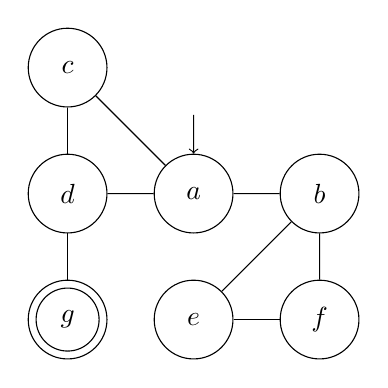
\begin{tikzpicture}[scale=0.8]
        % MDP i
        \node [draw, circle, minimum size=1cm] (a) at (2, 2) {$a$};
        \node [draw, circle, minimum size=1cm] (b) at (4, 2) {$b$};
        \node [draw, circle, minimum size=1cm] (c) at (0, 4) {$c$};
        \node [draw, circle, minimum size=1cm] (d) at (0, 2) {$d$};
        \node [draw, circle, minimum size=1cm] (e) at (2, 0) {$e$};
        \node [draw, circle, minimum size=1cm] (f) at (4, 0) {$f$};
        \node [draw, circle, minimum size=1cm] (g) at (0, 0) {$g$};
        \node [draw, circle, minimum size=0.8cm] at (0, 0) {};

        \coordinate[above of=a] (init);

        \draw[->] (init) -- (a);
        \draw[-] (a) -- (b);
        \draw[-] (a) -- (c);
        \draw[-] (a) -- (d);
        \draw[-] (b) -- (e);
        \draw[-] (b) -- (f);
        \draw[-] (c) -- (d);
        \draw[-] (d) -- (g);
        \draw[-] (e) -- (f);
        \draw[-] (d) -- (g);
    \end{tikzpicture}
    \caption{状態空間問題の例。エージェントはスタート地点$a$からゴール地点$g$を目指す。問題は\cite{edelkamp:2010:hst:1875144}より。
    }
	\label{fig:ssp-graph}
    % TODO: なんか面白そうにする
\end{figure}


\begin{figure}
	\centering
    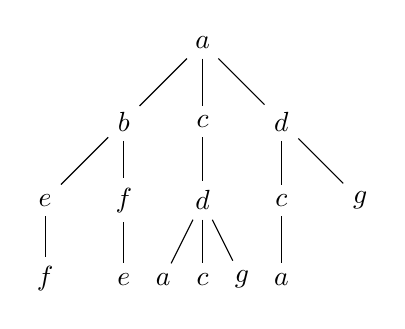
\begin{tikzpicture}[scale=0.5]
        % MDP i
        \node (a0) at (4, 6) {$a$};

        \node (b1) at (2, 4) {$b$};
        \node (c1) at (4, 4) {$c$};
        \node (d1) at (6, 4) {$d$};

        \node (e2) at (0, 2) {$e$};
        \node (f2) at (2, 2) {$f$};
        \node (d2) at (4, 2) {$d$};
        \node (c2) at (6, 2) {$c$};
        \node (g2) at (8, 2) {$g$};

        \node (f3) at (0, 0) {$f$};
        \node (e3) at (2, 0) {$e$};
        \node (a31) at (3, 0) {$a$};
        \node (c3) at (4, 0) {$c$};
        \node (g3) at (5, 0) {$g$};
        \node (a32) at (6, 0) {$a$};

        \draw[-] (a0) -- (b1);
        \draw[-] (a0) -- (c1);
        \draw[-] (a0) -- (d1);
        \draw[-] (b1) -- (e2);
        \draw[-] (b1) -- (f2);
        \draw[-] (c1) -- (d2);
        \draw[-] (d1) -- (g2);
        \draw[-] (d1) -- (c2);
        \draw[-] (e2) -- (f3);
        \draw[-] (f2) -- (e3);
        \draw[-] (d2) -- (a31);
        \draw[-] (d2) -- (c3);
        \draw[-] (d2) -- (g3);
        \draw[-] (c2) -- (a32);
    \end{tikzpicture}
    \caption{状態空間問題の経路木。エージェントはスタート地点$a$からゴール地点$g$を目指す。\\
    }
    \label{fig:ssp-tree}
\end{figure}

%\captionlistentry[todo]{状態空間問題の例示}

この本では主に初期状態とゴール条件が与えられたとき、ゴール条件を満たすための経路を返す問題を探索する手法を考える。
特に本書の主眼は\ref{ch:state-space-problem}章から\ref{ch:heuristic-search-variants}章までで扱う\define{状態空間問題}{state-space problem}{じょうたいくうかんもんだい}である。


\ddef{ユニットコスト状態空間問題、state-space problem}{
	ユニットコスト状態空間問題$P = (S, A, s, T)$は状態の集合$S$、初期状態$s \in S$、ゴール集合$T \in S$、アクション集合$A = {a_1, ....,a_n}$、$a_i : S \rightarrow S$が与えられ、初期状態$s$からゴール状態へ遷移させるアクションの列を返す問題である。
}

よって、ユニットコスト状態空間問題はグラフにモデルすることで考えやすくなる。
ユニットコスト状態空間問題を表す\define{状態空間グラフ}{state-space graph}{じょうたいくうかんぐらふ}は以下のように定義される。

\ddef{状態空間グラフ、State-space graph}{
問題グラフ$G = (V, E, s, T)$は状態空間問題$P = (S, A, s, T)$に対して以下のように定義される。ノード集合 $V = S$、初期ノード$s \in S$、ゴールノード集合$T$、エッジ集合$E\subseteq V \times V$。エッジ$u,v\in E$は$a(u) = v$となる$a\in A$が存在する場合に存在し、そしてその場合にのみ存在する(iff)。
}

状態空間問題の\define{解}{solution}{かい}は以下の定義である。

\ddef{解、Solution}{
解$\pi = (a_1,a_2...,a_k)$はアクション$a_i \in A$の(順序付)配列であり、初期状態$s$からゴール状態$t \in T$へ遷移させる。すなわち、$u_i \in S$,$i \in \{0,1,...,k\}$, $u_0 = s, u_k = t$が存在し、$u_i = a_i(u_{i-1})$となる。
}

どのような解を見つけたいかは問題に依存する。
多くの問題では\define{経路コスト}{path cost}{けいろこすと}の合計を小さくすることを目的とする。

%すなわち、アクションに対してコストが定義されており、経路

\ddef{状態空間問題、Weighted state-space problem}{
	状態空間問題$P = (S, A, s, T, w)$はユニットコスト状態空間問題の定義に加え、コスト関数$w: A \rightarrow \mathbb{R}$がある。経路$(a_1,...,a_k)$のコストは$\sum^k_{i=1}w(a_i)$と定義される。
}

%ある解が可能なすべての解の中でコストが最小である場合、その解を最適解(optimal cost solution)であると言う。
本書ではこの状態空間問題を主に扱う。
状態空間問題のうちコストが定数関数である場合がユニットコスト状態空間問題である。
状態空間問題は重み付き(コスト付き)グラフとしてモデルすることが出来る。すなわち、$G = (V, E, s, T, w)$は状態空間グラフの定義に加え、エッジの重み$w: E \rightarrow \mathbb{R}$を持つ。

\ref{ch:blind-search}章で詳解するが、探索アルゴリズムは状態空間グラフのノード・エッジ全てを保持する必要はない。
全てのノード・エッジを保持した状態空間グラフを特に\define{明示的状態空間グラフ}{explicit state-space graph}{めいじてきじょうたいくうかんぐらふ}と呼ぶとする。このようなグラフは、例えば隣接行列を用いて表すことが出来る。隣接行列$M$は行と列の大きさが$|V|$である正方行列であり、エッジ$(v_i, v_j)$が存在するならば$M_{i,j}=1$、なければ$M_{i,j}=0$とする行列である。
このような表現方法の問題点は行列の大きさが$|V|^2$であるため、大きな状態空間を保持することが出来ないことである。
例えば、\ref{sec:search-problem}節で紹介する15-puzzleは状態の数が$|V|=15!/2$であるため、隣接行列を保持することは現在のコンピュータでは非常に困難である。

そこで、探索アルゴリズムは多くの場合初期ノードとノード展開関数による\define{非明示的状態空間グラフ}{implicit state-space graph}{ひめいじてきじょうたいくうかんぐらふ}で表せられる。

\ddef{非明示的状態空間グラフ、Implicit state-space graph}{
	非明示的状態空間グラフは初期状態$s \in V$、ゴール条件Goal: $V \rightarrow B = \{false, true\}$、ノード展開関数Expand: $V \rightarrow 2^V$\footnote{$2^V$はノード集合$V$の冪集合である。}によって与えられる。
}


探索の開始時、エージェントは初期ノードのみを保持する。エージェントは保持しているノードに対してExpandを適用することによって、新しいノードとエッジをグラフに加える。これを求める解を見つけるまで繰り返す。
Expandはある状態からの可能な次の状態の集合を返す関数である。Expand関数は明示的に与えられるのではなく、ルールによって与えられることが多い。例えば将棋であれば、将棋のルールによって定められる合法手によって得られる次の状態の集合がExpand関数によって得られる。
これによって、エージェントは解を見つけるまでのノード・エッジだけ保持して必要な解を見つけることが出来る。


%\begin{example}

%\end{example}

%大まかには、情報なし探索による非明示的グラフは明示的グラフよりも指数的に小さく、ヒューリスティック探索による非明示的グラフは情報なし探索による非明示的グラフよりも更に指数的に小さいことが多い。

\begin{comment}
\section{状態空間問題の定式化}
\label{sec:search-problem-formulation}

状態空間問題の定式化の方法は様々である。
前述のように、状態空間$S$のすべての状態$s \in S$が陽に列挙されていることはあまりない。
多くの場合、状態は変数の列によって表せられる: $s = (v_0, v_1,...,v_n)$。これらの変数は状態変数と呼ぶこととする。これによって変数の組み合わせが状態空間となりグラフのノードを構成する。
そしてグラフのエッジはノード展開関数を用いて定義される。


\begin{table}
\caption{状態空間問題における問題の定式化。もっとも情報が多く与えられる定式化がドメイン依存エージェントであり、ヒューリスティック関数なども与えられる。ドメイン非依存エージェントはPDDLなどのモデル言語で書かれた入力が与えられ、その情報から用いるヒューリスティック関数や効率化手法を自動的に選択する必要がある。ブラックボックスエージェントは事前に何も与えられない、最も挑戦的な定式化である。}
\label{tbl:search-problem-formulation}
%\begin{adjustbox}{width=\textwidth}
\begin{tabular}{c|ccc}
	問題		& 状態遷移関数 	& ヒューリスティック関数 & 効率化 \\ \hline
	ドメイン依存 & Fully Available & hard-code & hard-code \\
	ドメイン非依存 (PDDL) & Fully Available & 自動生成する必要がある & ドメイン非依存の最適化・ポートフォリオ戦略 \\
	ブラックボックス & Unavailable (simulator) & Unavailable & 非許容的なノード・エッジの枝刈り
\end{tabular}
%\end{adjustbox}
\end{table}

% TODO: アルゴリズムを表にする?
\end{comment}


\section{状態空間問題の例}
\label{sec:search-problem}

状態空間問題の例をいくつか紹介する。
これらの問題はすべてヒューリスティック探索研究でベンチマークとして広く使われているものである。

%グリッド経路探索問題など、応用がありつつ、かつ分かりやすい問題を選んだ。
%グラフ探索アルゴリズムによって効率的に解くことが出来ると知られているドメインをいくつか紹介する。
%ここで詳解する問題はグラフ探索以外の手法でも解くことが出来る。


\subsection{グリッド経路探索 (Grid Path-Finding)}
%\captionlistentry[todo]{Grid Pathfinding: なんかいい感じの絵}
%{\TODO Grid Pathfinding: なんかいい感じの絵}


\define{グリッド経路探索問題}{grid path-finding problem}{グリッドけいろたんさくもんだい}は$k$(多くの場合$k=2$)次元のグリッド上で初期配置からゴール位置までの経路を求める問題である\cite{yap2002grid}。グリッドには障害物がおかれ、通れない箇所がある。エージェントが移動できる方向は4方向($A= \{up, down, left, right\}$)か8方向(4方向に加えて斜め移動)とする場合が多い。自由方向(Any Angle)の問題を扱う研究も存在する\cite{nash2007theta}。

\begin{figure}
        \centering
	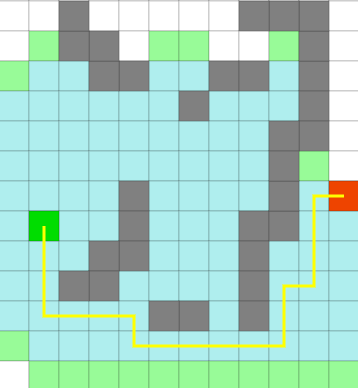
\includegraphics[width=0.5\textwidth]{figures/grid-astar.png}
	\caption{グリッド経路探索問題}
	\label{fig:grid-pathfinding}
\end{figure}


Web上に簡単に試せるデモがあるので、参照されたい\footnote{\url{http://qiao.github.io/PathFinding.js/visual/}}。この本の画像の一部はこのデモをもとに作成している。この本で説明する様々なグラフ探索手法をグリッド経路探索に試すことが出来る。

グリッド経路探索はロボットのモーションプランニングやゲームAIなどで応用される\cite{algfoor2015comprehensive}。ストラテジーゲームなどでユニット(エージェント)を動かすために使われる \cite{cui2011based}。よく使われるベンチマーク問題集にもStarcraftのゲームのマップが含まれている\cite{sturtevant2012benchmarks}.
またグリッドは様々な問題を経路探索に帰着して解くことができるという意味でも重要である。例えば多重整列問題 (Multiple Sequence Alignment)はグリッド経路探索に帰着して解くことが出来る(後述)。
ロボットのモーションプランニングも経路探索に帰着することが出来る \cite{barraquand91}。すなわち、$k$個の関節の角度を変えて、現在状態からゴール状態へ遷移させたい。各関節の角度がグリッドの各次元に相当する。ロボットの物理的な構造により、関節のある角度の組み合わせは不可能である。不可能な組み合わせが、障害物の置かれたグリッドに相当する。よって、障害物を避けた経路というのが関節の動かし方ということになる。

%Starcraft 1ではA*探索が使われていた。
%しかしマルチエージェント
%マルチエージェント経路探索の場合はflocking / swarm AIが使われている。Starcraft 2では


\subsection{スライディングタイル (Sliding-tile Puzzle)}

多くの一人ゲームはグラフ探索問題に帰着することが出来る。スライディングタイルはその例であり、ヒューリスティック探索研究においてメジャーなベンチマーク問題でもある (図\ref{fig:15-puzzle}) \cite{johnson1879notes}。
$1$から$(n^2)-1$までの数字が振られたタイルが$n\times n$の正方形に並べられている。正方形には一つだけ{\it ブランク}と呼ばれるタイルのない位置があり、四方に隣り合うタイルのいずれかをその位置に移動する(スライドする)ことが出来る。スライディングタイル問題は、与えられた初期状態からスライドを繰り返し、ゴール状態にたどり着く経路を求める問題である。

\begin{figure}
\centering
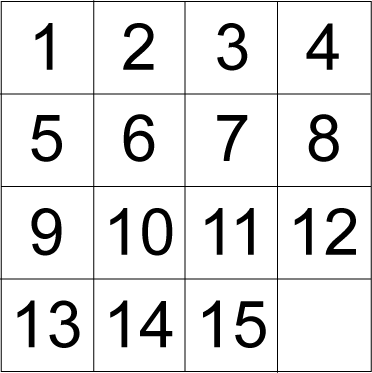
\includegraphics[bb=0 0 372 373,width=0.5\textwidth]{figures/15-puzzle.png}
\caption{15パズルのゴール状態の例}
\label{fig:15-puzzle}
\end{figure}


スライディングタイルの到達可能な状態の数は$|V| = (n^2)!/2$\footnote{スライディングタイルは偶奇性があり、到達不可能な状態がある\cite{johnson1879notes}。}であり、$n$に対して指数的に増加する。
可能なアクションは$A= \{up, down, left, right\}$の4つであり、アクションにかかるコストはすべて同じとする。

後述するが、ヒューリスティック探索のためには状態からゴール状態までの距離(コスト)の下界(lower bound)が計算できると有用である。
スライディングタイルにおける下界の求め方として最もシンプルなものは{\it マンハッタン距離ヒューリスティック}である。マンハッタン距離ヒューリスティックは各タイルの現在状態の位置とゴール状態の位置のマンハッタン距離の総和を取る。可能なアクションはすべて一つしかタイルを動かさないので、一回のアクションでマンハッタン距離は最大で1しか縮まらない。よって、マンハッタン距離はゴールまでの距離の下界である。

%ちなみに、スライディングタイルはpermutation problemの一つである。

\subsection{多重整列問題 (Multiple Sequence Alignment)}
\label{sec:msa}
生物学・進化学では遺伝子配列・アミノ酸配列の編集距離(edit distance)を比較することでニ個体がどれだけ親しいかを推定することが広く研究されている。
\define{多重整列問題}{Multiple Sequence Alignment}{たじゅうせいれつもんだい} (MSA)は複数の遺伝子・アミノ酸配列が与えられた時、それらの配列間の編集距離とその時出来上がった配列を求める問題である。
2つの配列に対してそれぞれコストの定義された編集操作を繰り返し、同一の配列に並べ替える手続きをアライメントと呼ぶ。
2つの配列の編集距離は編集操作の合計コストの最小値である。
3つ以上の配列における距離の定義は様々考えられるが、ここでは全ての配列のペアの編集距離の総和を用いる。

MSAにおける可能な編集操作は置換と挿入である。置換は配列のある要素(DNAかアミノ酸)を別の要素に入れ替える操作であり、挿入は配列のある位置に要素を挿入する操作である。例えば(ABC, BCB, CB)の3つの配列のアライメントを考える。図\ref{fig:msa-cost}は置換と編集に対するコストの例である。-は欠損、すなわち挿入操作が行われたことを示す。アミノ酸配列における有名なコスト表としてPAM250\cite{pearson1990}があるが、ここでは簡単のため仮のコスト表を用いる。
図\ref{fig:msa-solution}はこのコスト表を用いたアライメントの例である。
このとき、例えば配列ABC-と-BCBの編集距離は(A,-)、 (B,B)、 (C,C)、 (-,B)のコストの総和であるので、図\ref{fig:msa-cost}を参照し、$5+0+1+5=11$である。(-BCB, --CB)の距離は$6$, (--CB, ABC-)の距離は$16$であるので、3配列の編集距離は$11+6+16=33$である。

$n$配列のMSAは$n$次元のグリッドの経路探索問題に帰着することが出来る\cite{korf:2000}。
図\ref{fig:msa-to-grid}は(ABC)と(BCB)の2つの配列による問題を表す。
状態$s$は2つの変数によって表現される:$(x_0, x_1)$。$x_0$は配列0のどの位置までアライメントを完了したかを表す変数であり、配列$i$の長さを$l_i$とすると定義域は$0 \leq x_0 \leq l_0$である。
全てのアライメントが完了した状態$s=(l_0, l_1)$がゴール状態である。
可能なアクションは$a=(b_0, b_1), (b_i=0, 1)$の形を取り、これは配列$i$に対して欠損を挿入する場合に$b_i=0$となる。
状態$s$に対してアクション$a$を適用した後の状態$s'$は$s'=(x_0+b_0, x_1+b_1)$となる。例えば図\ref{fig:msa-to-grid}は初期状態$s=(0,0)$に対して$a=(1,0)$を適用している。これは(A), (-)までアライメントを進めた状態に対応する。次に$a=(1,1)$が適用され、アライメントは(A,B), (-,B)という状態に至る。

このようにして、MSAはグリッド経路探索問題に帰着し、グラフ探索アルゴリズムよって解くことが出来る。
状態空間問題として考えた場合にMSAの難しさはアクションのコストが幅広いことにある。また、可能なアクションの数も配列の数$n$に対して$2^n-1$と大きい。

MSAは生物学研究に役立つというモチベーションから非常に熱心に研究されており、様々な定式化による解法が知られている。
詳しくは\cite{waterman1995introduction,
gusfield1997algorithms,edgar2006multiple}を参照されたい。


\begin{figure}
\centering
\includegraphics[width=0.95\textwidth]{figures/msa.png}
\caption{多重整列問題: 画像はwikipediaより。}
\label{fig:msa-gif}
\end{figure}


\begin{figure}
\centering
\subfloat[MSAの解の例]{
\begin{tabular}{ccccc}
	A & B & C & - \\
	- & B & C & B \\
	- & - & C & B \\
\end{tabular}
\label{fig:msa-solution}
} \hspace{4pt}
\subfloat[操作コスト表の例]{
\begin{tabular}{c|cccc}
	  & A & B & C & - \\ \hline
	A & 0 & 1 & 2 & 5 \\
	B &   & 0 & 3 & 5 \\
	C &   &   & 1 & 5 \\
	- &   &   &   & 0 \\	
\end{tabular}
\label{fig:msa-cost}
} \hspace{4pt}
\subfloat[グリッド経路探索への帰着]{
\begin{tabular}{c|cccc}
	  &   & A & B & C \\ \hline
	  & $\rightarrow$ & $\searrow$ &   &   \\
	B &   &   & $\searrow$ &   \\
	C &   &   &   & $\downarrow$ \\
	B &   &   &   & $\searrow$ \\
\end{tabular}
\label{fig:msa-to-grid}
}
\subfloat[グリッド経路探索への帰着]{
\begin{tabular}{c|cccc}
	  & A & B & C & - \\ \hline
	  & - & B & C & B \\ \hline
\end{tabular}
\label{fig:msa-to-grid-align}
}
\end{figure}


\subsection{倉庫番 (Sokoban)}
倉庫番(Sokoban)は倉庫の荷物を押していくことで指定された位置に置くというパズルゲームである。現在でも様々なゲームの中で親しまれている \cite{junghanns1997sokoban,culberson:97}。
プレイヤーは「荷物の後ろに回って押す」ことしか出来ず、引っ張ったり、横から動かしたりすることが出来ない。また、荷物の上を通ることも出来ない。
PSPACE-completeであることが知られている\cite{culberson:97}。

\begin{figure}
\centering
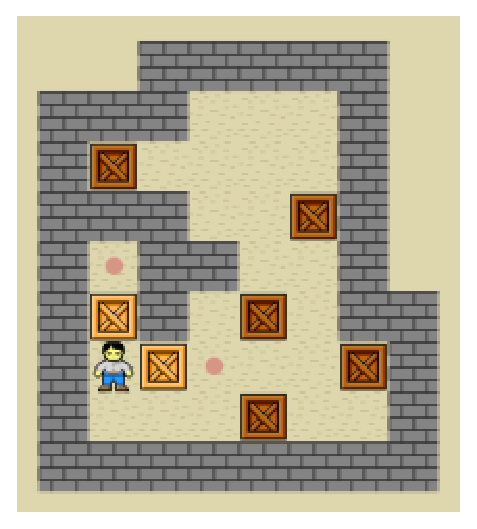
\includegraphics[bb=0 0 213 238,width=0.5\textwidth]{figures/sokoban.eps}
\caption{Sokoban: 画像はwikipediaより。}
\label{fig:sokoban}
\end{figure}

状態の表現方法は2通りあり、一つはグリッドの各位置に何が置いてあるかを変数とする方法である。もうひとつはプレイヤー、各荷物の位置に対してそれぞれ変数を割り当てる方法である。
可能なアクションは{\tt move-up}, {\tt move-left}, {\tt move-down}, {\tt move-right}, {\tt push-up}, {\tt push-left}, {\tt push-down}, {\tt push-right} の8通りである。{\tt move-*}はプレイヤーが動くアクションに対応し、コストは0である。{\tt push-*}は荷物を押すアクションであり、正のアクションコストが割当てられている。よって、倉庫番はなるべく荷物を押す回数を少なくして荷物を目的の位置に動かすことが目的となる。

グラフ探索問題として倉庫番を考えるときに重要であるのは、倉庫番は{\it 不可逆な}アクション(irreversible)があることである。
グリッド経路探索やスライディングタイルは{\it 可逆な} (reversible)問題である。
全てのアクション$a \in A$に対して$a^{-1} \in A$が存在し、$a(a^{-1}(s)) = s$かつ$a^{-1}(a(s)) = s$となる場合、問題は可逆であると言う。
可逆な問題は対応するアクションのコストが同じであれば無向グラフとしてモデルすることも出来、初期状態から到達できる状態は、すべて初期状態に戻ることが出来る。
一方、不可逆な問題ではこれが保証されず、詰み(trap)状態に陥る可能性がある (\ref{sec:difficulity}節)。

倉庫番では荷物を押すことは出来ても引っ張ることが出来ないため、不可逆な問題である。例えば、荷物を部屋の隅に置いてしまうと戻すことが出来ないため、詰み状態に陥る可能性がある問題である。
このような性質を持つ問題では特にグラフ探索による先読みが効果的である。

もうひとつ重要な問題は\define{ゼロコストアクション}{zero-cost action}{ゼロコストアクション}の存在である。ゼロコストアクションはコストが0のアクションである。%TODO
倉庫番のアクションのうち{\tt move-up}, {\tt move-left}, {\tt move-down}, {\tt move-right}はコストゼロ($w(e)=0$)のアクションである。ヘタなアルゴリズムを実行すると無限に無駄なアクションを繰り返し続けるということもありうるだろう。


%倉庫の中には荷物がおかれ、エージェント(プレイヤー)は迷路を動き回り、
%このゲームで面白い/難しいのは、「荷物の後ろに回って押す」ことしか出来ず、引っ張ったり、横から動かしたりすることが出来ないという点である。

\subsection{巡回セールスパーソン問題 (Traveling Salesperson Problem, TSP)}

セールスパーソンはいくつかの都市に回って営業を行わなければならない。都市間の距離(=コスト)は事前に与えられている。
TSPは全ての都市を最短距離で回ってはじめの都市に戻る経路を求める、という問題である\cite{applegate2006traveling}。

\begin{figure}
\centering
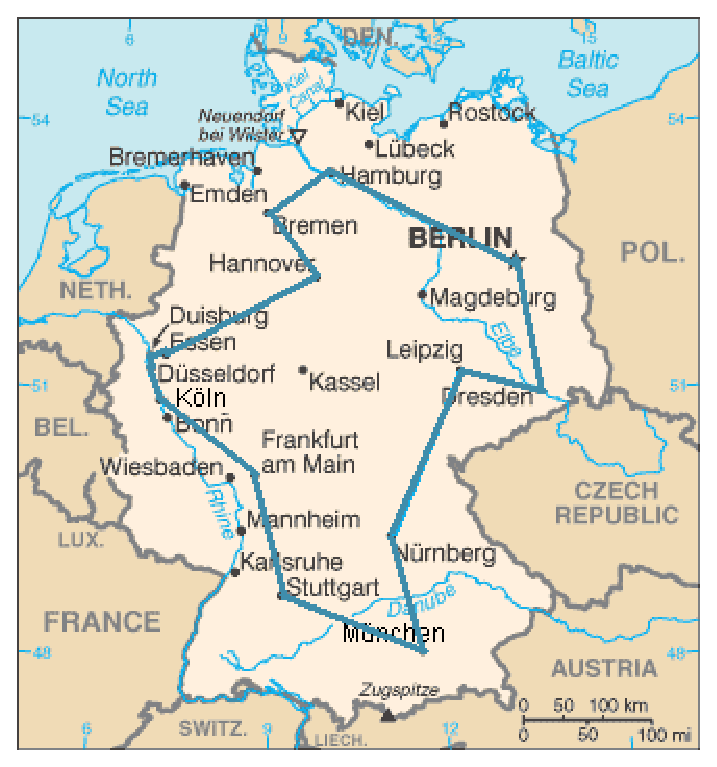
\includegraphics[bb=0 0 328 352,width=0.5\textwidth]{figures/tsp.eps}%TODO
\caption{巡回セールスパーソン問題: 画像はwikipediaより。}
\label{fig:sokoban}
\end{figure}

$n$個の都市があるとすると(最適・非最適含む)解の数は$(n-1)!/2$個である。
可能なアクションは「都市$i \in \{1..n\}$を訪れる」であり、一度訪れた都市には行けない。
TSPのゴール条件はすべての都市を訪れることである。よって、$n$回どれかアクションを実行すれば、とりあえず解を得ることが出来る。一方、最適解を得る問題はNP完全であることが知られている。

TSPの解の下界としては{\it 最小全域木} (minimum spanning tree)のコストがよく用いられる\cite{kruskal1956shortest,held1970traveling}。
グラフの{\it 全域木} (spanning tree)は全てのノードを含むループを含まない部分グラフである。
最小全域木は全域木のうち最もエッジコストの総和が小さいものである。
未訪問の都市によるグラフの最小全域木はTSPの下界となることが知られている。

TSPはヒューリスティック探索に限らず、様々なアプローチで研究されている問題ドメインである\cite{applegate2006traveling}。TSPについて特に詳しく知りたい方はそちらの教科書を参照されたい。


%\subsection{ペネトレーションテスト}

%\subsection{モデル検査}


\section{問題の性質・難しさ}
\label{sec:difficulity}
% TODO: どこにこの章を置くべきか?
% この節は最初に読む際は飛ばすべきである。

本書で定義した状態空間問題は小さなモデルである。
完全情報であり、状態遷移は決定論的である。
% 最小コスト経路探索は
それでもNP困難問題であり、難しい問題は難しい。
この節は問題の難しさがどのような要素に左右されるかを列挙する。

\begin{enumerate}
\item {\bf 状態空間の大きさ}

状態空間の大きさ$|S|$は大きい程概して問題は難しくなる。
特に状態空間が無限である場合深さ優先探索などのアルゴリズムは停止しない場合がある。
例えば状態変数に実数が含まれる場合、状態空間の大きさは無限になる。
% 状態空間の大きさがそのまま問題の難しさに直結するわけではない。

\item {\bf 分枝度}

ある状態$s$の\define{分枝度}{branching factor}{ぶんしど}はそのノードの子ノードの数を指す。
特に状態空間問題の分枝度は、すべての状態の分枝度の平均を指す。ただし多くの場合平均を厳密に求めることはなく、おおよその平均を指して分枝度をすることが多い。
分枝度が大きいほど問題は難しいとは限らない。
分枝度が多いほどグラフが密である、つまりエッジの数が多いことに対応する。
%エッジが多い程解の候補となる経路が多くなる。
分枝度を$b$とすると、あるノード$s$の子ノードの数は$b$個であり、孫ノードの数は$b^2$である。$s$からの深さ$d$のノードは$b^d$個である。

\item {\bf デッドエンド}

問題によってはある状態に到達するともう問題を解くことは出来ないというシチュエーションがある。例えば倉庫番は荷物を角においてしまうともう動かすことができない。これによってもう問題がクリアできなくなるということがある。このような問題では状態空間を広く探索し、デッドエンド状態のみを探索し続けるということをうまく避ける必要がある。例えば\ref{sec:greedy-best-first-search}節の貪欲最良優先探索はデッドエンドに入ってしまうとなかなか抜け出せないかもしれない。
% あるいはデッドエンドを検知する手法も考えられる。
概してデッドエンドがある問題では状態空間を広く探索する手法、探索済みの状態を記録する手法が有利であり、局所探索手法はうまくいかないことがある。
%このような問題では局所探索アルゴリズムではうまくいかないことがある。局所探索アルゴリズムは

\item {\bf 解の存在}

当然解が存在しない問題もありうる。
本書で紹介するアルゴリズムは解が存在しない場合非常に時間がかかるものが多い\footnote{一般にどのようなアルゴリズムを使っても解が存在しない状態空間問題は難しい。}。
一部のアルゴリズムは解が存在しない場合永遠に停止しない場合がある。
そのような場合、アルゴリズムは解が存在しないと示せれば理想的である。
そのため解が存在しないことを検出するアルゴリズムの研究もされている \cite{backstrom2013fast,hoffmann2014distance}。

\end{enumerate}

\section{関連文献}

本章で定義した状態空間問題は基本となる定義であり、完全情報であり状態遷移が決定論的であることを仮定した。
状態遷移が決定論的ではなく確率的であると仮定したモデルは\define{マルコフ過程問題}{Markov Decision Process Problem}{マルコフかていもんだい} (MDP)と呼ばれている。
状態空間問題はMDPの特殊な場合である。
%図\ref{fig:mdp}のようにマルコフ過程問題もグラフによってモデルすることができる。
%グラフのノードは2種類あり、状態を表すノードと状態とアクションのペアを表すノードがある。
%状態とアクションのペアを表すノードからは可能な遷移先へのエッジが伸びている。また、このエッジには遷移確率のラベルがついている。
MDPは\define{強化学習}{reinforcement learning}{きょうかがくしゅう}における問題モデルとしても広く使われている。
MDPにおけるプランニング問題を解くためにはグラフ探索アルゴリズムも使えるが、動的計画法も用いられる \cite{puterman2014markov}。
MDPからさらに不完全情報問題に拡張したものを\define{部分観測マルコフ過程問題}{partially observable Markov decision process problem}{ぶぶんかんそくマルコフかていもんだい} (POMDP)と呼ぶ。
POMDPにおけるプランニング問題の厳密解はBelief spaceプランニング \cite{kaelbling1998planning}によって求められるが、多くの場合計算困難(intractable)であるので近似手法が用いられる。

%状態遷移が他のエージェントによるアクションによって左右される問題をマルチエージェント問題と呼ぶ。特に将棋、囲碁やチェスなどの敵対二人ゲームはグラフ探索が活躍するドメインである。

本書では状態空間問題の解をゴールに到達するまでの経路と定義した。
状態空間問題のもう一つの定式化として、状態とアクションの組に対して\define{報酬}{reward}{ほうしゅう} ($R: (S, A) \rightarrow \mathbb{R}$)を定義し、報酬を最大化する経路を求める問題がある。この定式化は特に強化学習で用いられる。

%状態空間問題の例としては\define{モデル検査}{model checking}がある。
%モデル検査はXXXYYY



